\section{Untersuchung optischer Elemente}
	
	\subsection{Methoden}
		
			\begin{figure}[ht]
				\centering
				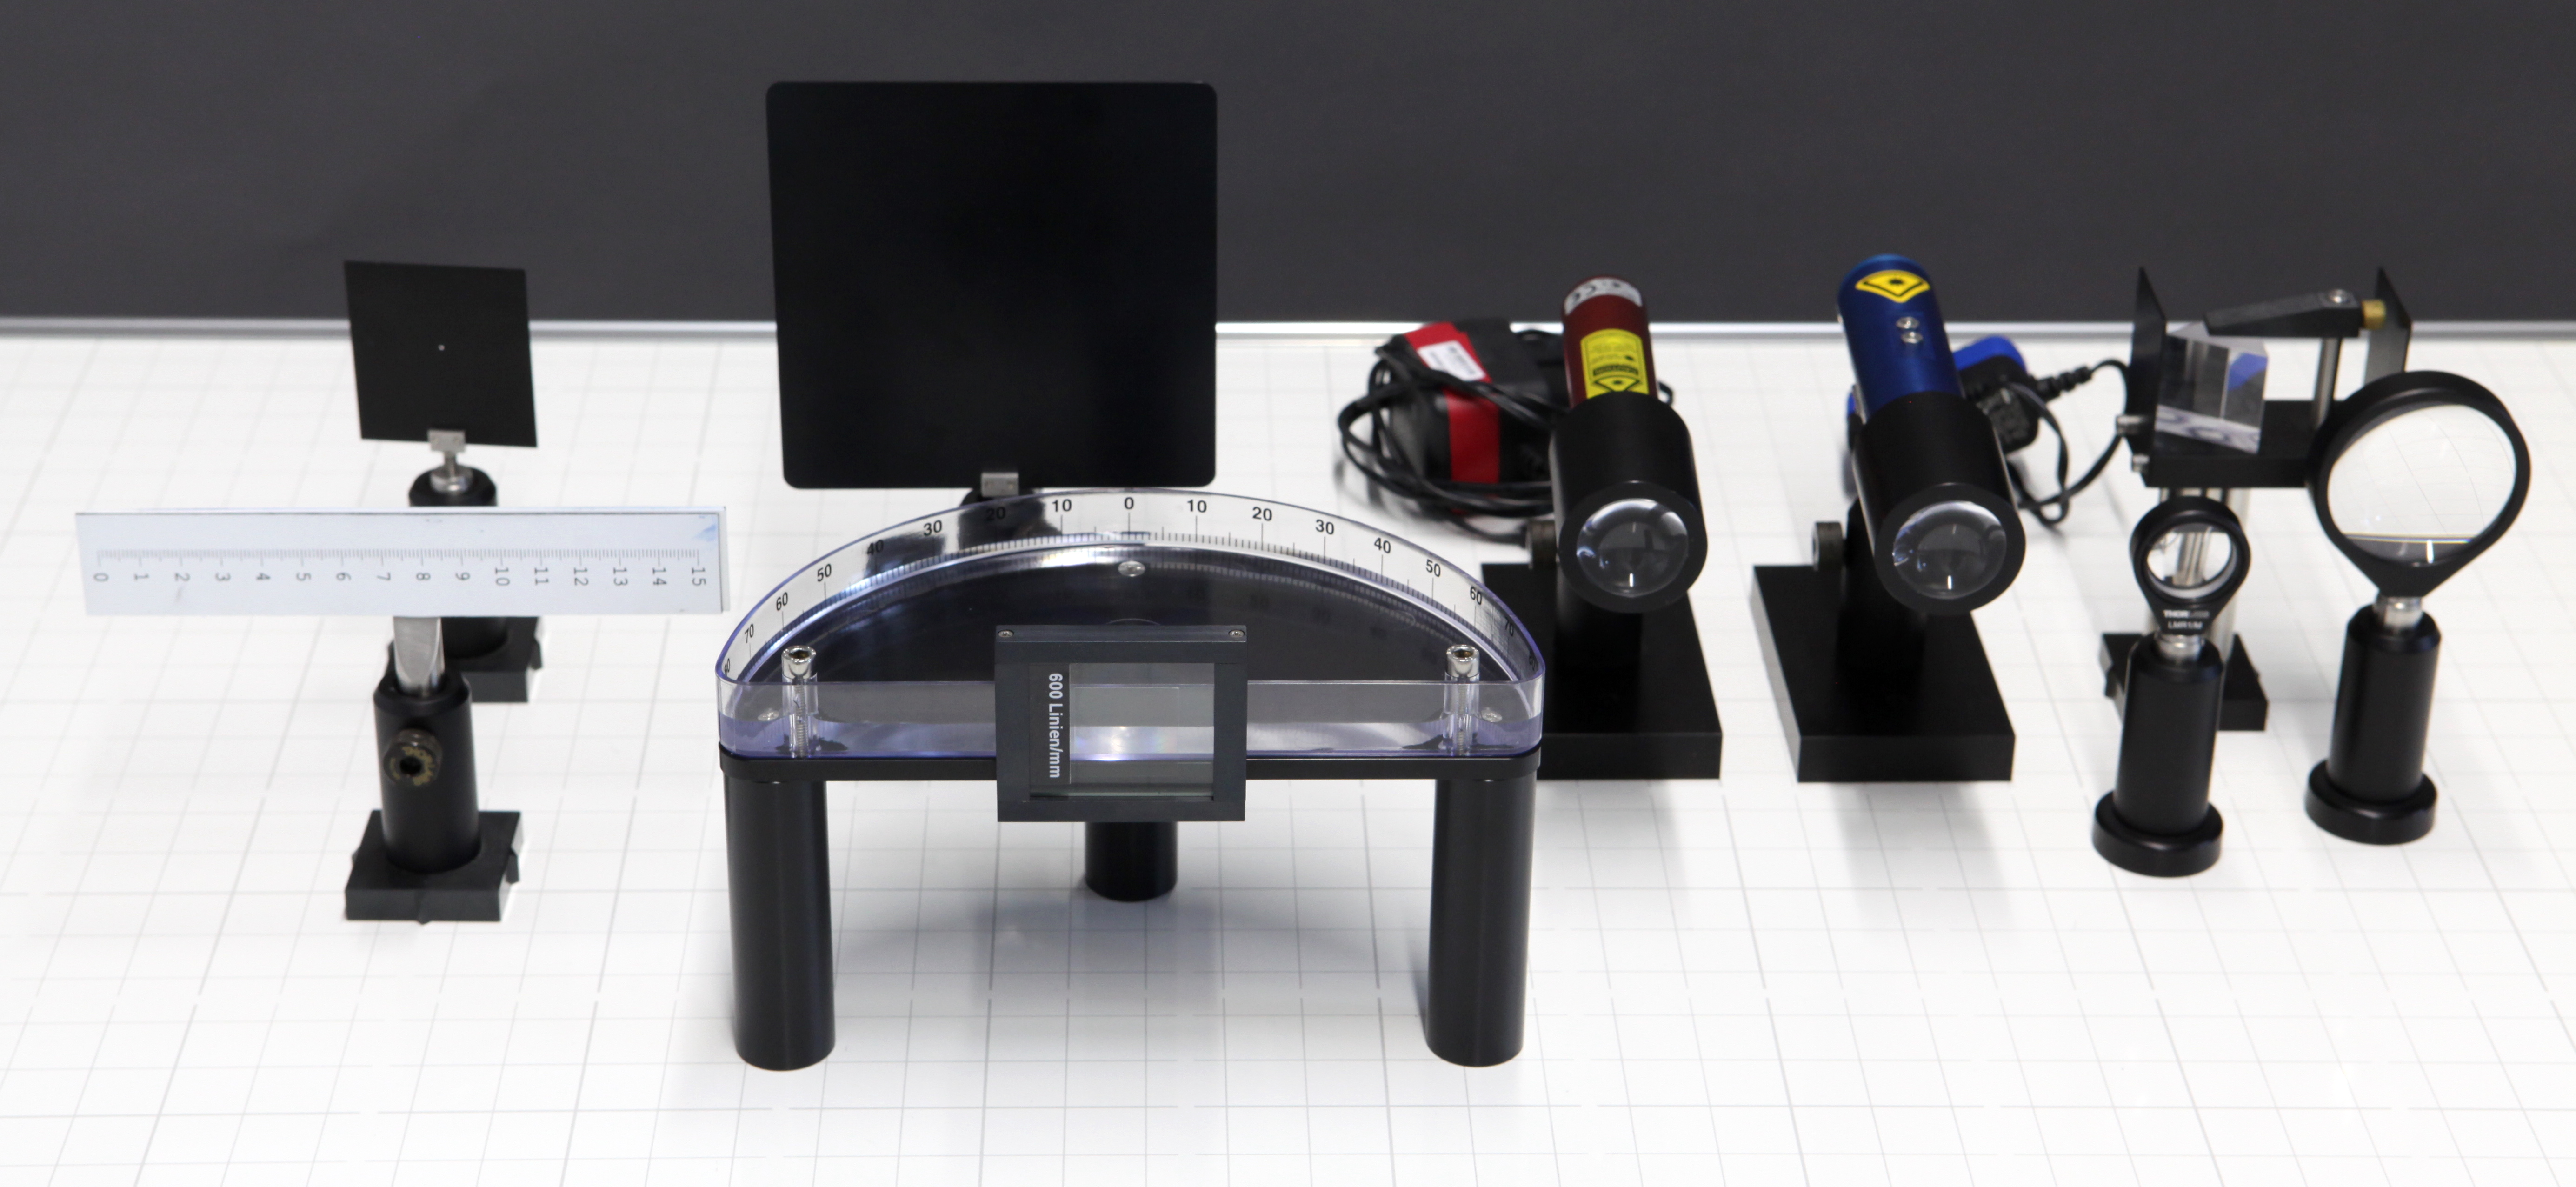
\includegraphics[width=\textwidth]{bilder/aufbau2.jpg}
			 	\caption{Für den Versuch verwendete Materialien.\cite{WWU}}
			 	\label{fig:Aufbau2}	
			\end{figure}
			Abbildung \ref{fig:Aufbau2} zeigt die für diesen Versuch verwendeten Materialien.
			Alle dieser befinden sich auf einer magnetischen Unterlage, sodass diese nicht einfach während der Messung verrutschen können.
			Zu den Materialien gehören ein roter Laser ($\lambda = \SI{650}{\nano\meter}$), ein blauer Laser ($\lambda = \SI{405}{\nano\meter}$) und eine Lochblende zur Ausrichtung eines geraden Strahlengangs, welcher parallel zu dem Raster auf der magnetischen Unterlage verlaufen soll.
			Für beide Laser soll dieser durch das Prisma und das Gitter verlaufen und für einen einzelnen durch die Linsen.
			
			Das Prisma besteht aus Flintglas und besitzt von vorne betrachtet die Form eines gleichseitigen Dreiecks ($\alpha = \SI{60}{\degree}$).
			Die Strahlen der beiden Laser sollen so gerichtet werden, dass sie durch den Apex des Prismas verlaufen.
			Als Schirm zur Messung der Ablenkung dient die horizontal ausgerichtete Messleiste.
			Zu beobachten ist die Änderung der Ablenkung bei dem Drehen des Prismas.
			Bei symmetrischem Strahlengang ist die Ablenkung minimal.
			Aus Abstand zur Messleiste $h$ und Ablenkung $x$ von der Nulllage (keine Ablenkung) lässt sich über
			\begin{equation}
				\tan \delta_m = \frac{h}{x} \Leftrightarrow \delta_m = \arctan \frac{h}{x}
			\end{equation}
			der minimale Ablenkwinkel $\delta_m$ bestimmen.
			\begin{figure}[ht]
				\centering
				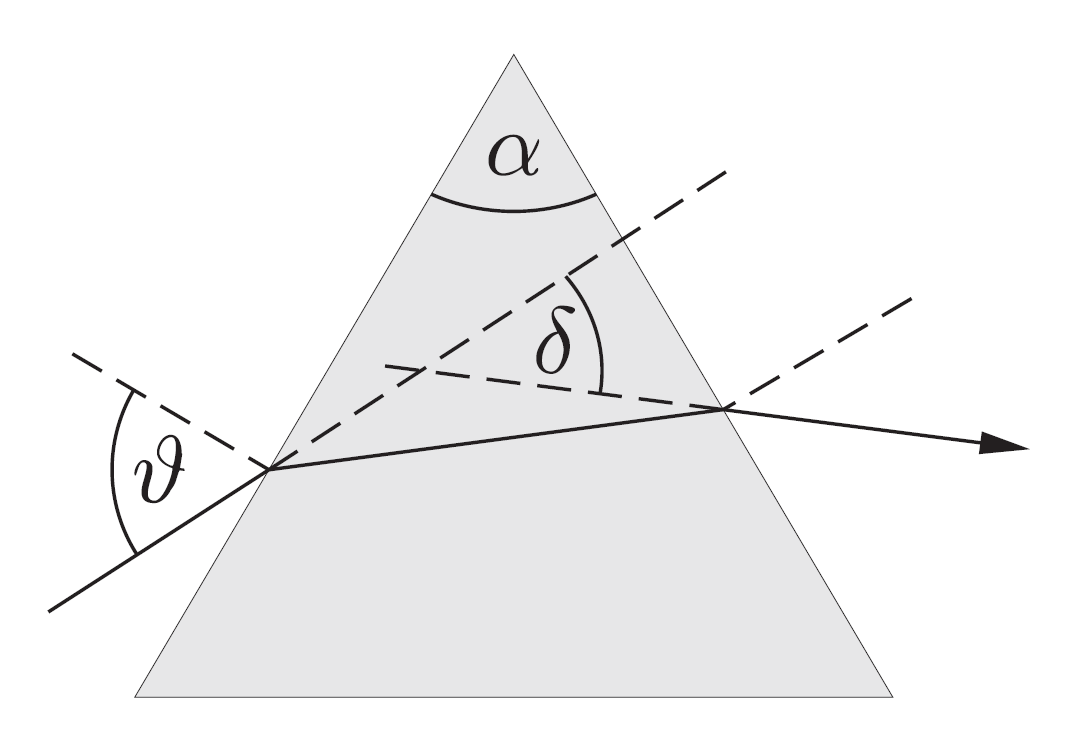
\includegraphics[width=0.5\textwidth]{bilder/prisma.png}
				\caption{Durchgang eines Lichtstrahls durch ein Prisma.\cite{WWU}}
				\label{fig:Prisma}	
			\end{figure}
			Zur Veranschaulichung dient Abb. \ref{fig:Prisma}.
			Für den symmetrischen Durchgang des Lichtstrahls durch das Prisma entfällt das $\vartheta$ in der Skizze und  es lässt sich für den Brechungsindex $n_\text{Prisma}$ des Prismas folgendes aufstellen:
			\begin{equation}
				n = \frac{\sin[(\delta_m + \alpha) / 2]}{\sin [\alpha / 2]}.
			\end{equation} 
			
			Das Gitter ist an einem offenen flachen Halbzylinder bzw. einer Halbkreisküvette angebracht, sodass die Ablenkung des Strahlengangs auf dem Gradmaß zu messen ist, welches auf der Innenseite dieser Küvette angebracht ist.
			Da diese offen ist, lässt sie sich mit einem anderem Material, hier destilliertes Wasser, füllen und daher eine andere Ablenkung des Strahls auf dem Gradmaß messen.
			An dieser Stelle lässt sich der Brechungsindex $n_\text{Wasser}$ des destillierten Wassers über das Snelliussche Brechungsgesetz $n_\text{Wasser} \sin \alpha_\text{Wasser} = n_\text{Luft} \sin \alpha_\text{Luft}$ bestimmen.
			
			Für die Linsen soll zunächst herausgefunden werden, um welche Typen es sich handelt.
			Dazu wird die Ablenkung des Laserstrahls bei den einzelnen Linsen betrachtet.
			An dieser Stelle soll zudem die Brennweite der Sammellinse bestimmt werden.
			Um diese zu bestimmen wird der Schirm verwendet und der Abstand von der Linse gesucht, bei dem alle Strahlen sich in einem Punkt treffen, auf dem Schirm der Laser also am kleinsten ist. 
			Danach sollen die Linsen so kombiniert werden, dass der Strahl vergrößert wird und dabei noch kollimiert ist.
			Hierfür ist der richtige Abstand zwischen den Linsen relevant.
			Aus diesem und der Brennweite der Sammellinse lässt sich die Brennweite der Streulinse einfach dadurch ermitteln, dass beide Brennpunkte aufeinander liegen müssen.  
			Zuletzt soll noch betrachtet werden wie sich der Strahlengang bei Drehung und Verkippung der Sammellinse verhält, wenn der Strahl mit einer Strahlenaufweitung aufgeweitet wird.
			
	\subsection{Durchführung}
		
		% TODO
		 
	\subsection{Datenanalyse}
		
		% TODO
		
	\subsection{Diskussion}
		
		Auch hier stellt sich nun die Frage, ob die Ziele der Untersuchung erreicht wurden.
		% TODO
		